\begin{frame}[allowframebreaks]{Key Components and Architectures}
    \begin{itemize}
        \item Autoregressive models are a class of statistical models where observations from previous time steps are used to predict the value at the current time step.
        \item They are commonly used for analyzing and forecasting time series data.
        \item The core principle is that the current value of a time series can be explained by its past values.
    \end{itemize}

    \begin{figure}
    \centering
    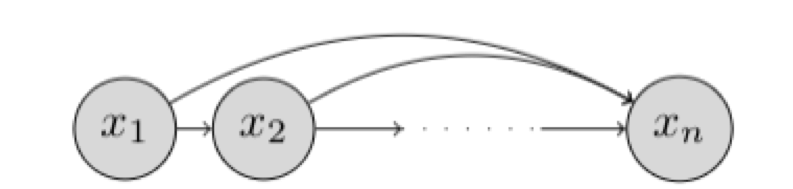
\includegraphics[height=0.5\textheight, width=\textwidth, keepaspectratio]{images/arm/autoregressive.png}
    \caption{Graphical model for an autoregressive network}
\end{figure}

\framebreak

\begin{itemize}
    \item In the MNIST dataset example, we can set an ordering for all the random variables from top-left $X_1$ to bottom-right $X_{784}$
    \item Without loss of generality, we can use chain rule for factorization
    $$\mathcal{P}(x_1, \cdots, x_{784}) = \mathcal{P}(x_1) \mathcal{P}(x_2|x_1) \mathcal{P}(x_3|x_1, x_2) \cdots \mathcal{P}(x_{784}|x_1, x_2, \cdots, x_{784})$$
    \item Parameterizing the above and using the sigmoid function for binarization,
    \begin{itemize}
        \item $\mathcal{P}_{CPT}(X_1=1;\alpha^1) = \alpha^1, \mathcal{P}(X_1=0) = 1-\alpha^1$
        \item $\mathcal{P}_{logit}(X_2=1|x_1;\alpha^2) = \sigma (\alpha_0^2 + \alpha_1^2 x_1)$
        \item $\mathcal{P}_{logit}(X_3=1|x_1,x_2;\alpha^3) = \sigma (\alpha_0^3 + \alpha_1^3 x_1 + \alpha_2^3 x_2)$
    \end{itemize}
\end{itemize}
\end{frame}